% Traversal-Based Relative Positional Encodings for Graph Neural Networks
% ACL 2023 template. Drop acl.sty / acl_natbib.bst alongside this file, or open the
% Overleaf ACL 2023 proceedings template and replace main.tex with this file.
%
% BUILD: pdflatex -> bibtex -> pdflatex -> pdflatex
%
% All sections are written. Every table and figure is generated by
% shared/07_results_and_figures.ipynb and copied in next to this file; nothing below is
% transcribed by hand. To refresh the numbers, re-run that notebook and re-copy:
%     paper_tables/table1_main.tex          -> Table 1
%     paper_tables/table2_expressivity.tex  -> Table 2
%     figures/fig_ablations.pdf             -> Figure 2
%     figures/fig_efficiency.pdf            -> Figure 3
%     figures/fig_distance_profile.pdf      -> Appendix A
% The only thing left to fill by hand is the repository URL in Appendix B.

\documentclass[11pt]{article}
\usepackage[]{acl}
\usepackage{times}
\usepackage{latexsym}
\usepackage[T1]{fontenc}
\usepackage[utf8]{inputenc}
\usepackage{microtype}
\usepackage{amsmath,amssymb,amsthm}
\usepackage{graphicx}
\usepackage{booktabs}
\usepackage{multirow}
\usepackage{url}

\newtheorem{proposition}{Proposition}
\newcommand{\WL}{\textsc{1-wl}}
\newcommand{\SPD}{\textsc{spd-wl}}
\newcommand{\SPC}{\textsc{spc-wl}}
\newcommand{\TRPE}{\textsc{t-rpe}}

\title{Traversal-Based Relative Positional Encodings\\for Graph Neural Networks}

\author{
  Chen Mizrahi \and Tomer Zalberg \and Ofek Tovli \and Itay Korenfeld \\
  Tel Aviv University \\
  \texttt{\{chenmizrahi,tomerzalberg,ofektovli,itaykorenfeld\}@mail.tau.ac.il}
}

\begin{document}
\maketitle

\begin{abstract}
Message-passing graph neural networks are bounded by the 1-Weisfeiler--Leman test, and
positional encodings are the standard remedy. Traversal-based encodings are almost always
\emph{absolute}: a node is described by its distance to a few anchors, inheriting whatever
arbitrariness chose them. We study the \emph{relative} alternative, a function of a node
\emph{pair}. Since every edge of a sparse graph joins nodes at distance one, such an encoding
is meaningful only on a rewired graph, so we attach the sinusoidally encoded hop distance
$d(u,v)$ to every pair within $r$ hops and inject it into GCN and GAT. We place the result
exactly in the expressiveness hierarchy---strictly above 1-WL, no stronger than 3-WL, strictly
strengthened by counting shortest paths---each claim confirmed on an explicit witness, the last
found by exhaustive search and shown to be minimal. Expressive power is not enough: on a
vertex-transitive graph with uniform features the normalised aggregation of both GCN and GAT
algebraically cancels any edge weighting, so an encoding injected that way provably cannot
help, and empirically scores exactly chance. Our pre-registered prediction that the encoding
helps on sparse, long-diameter graphs failed in the opposite direction---our largest gain
($+21.3$ points) is on the dataset we predicted would be degenerate---and the architecture,
not the graph, decides whether it helps at all.
\end{abstract}

\section{Introduction}

Message-passing graph neural networks (MPNNs) aggregate information over local neighbourhoods,
and their ability to distinguish graphs is bounded by the 1-Weisfeiler--Leman colour refinement
test \citep{xu2019gin,morris2019wlgo}. The bound is not a technicality: it means an MPNN cannot
see global symmetry, cannot measure how far apart two nodes are, and cannot separate graphs
that agree locally but differ globally.

Positional encodings (PEs) are the standard response. They enrich node features with a
structural signal computed outside the message-passing recursion, and they come in two
families. \emph{Absolute} PEs assign a vector to each node---Laplacian eigenvectors
\citep{dwivedi2023benchmarking,dwivedi2021generalization}, random-walk return probabilities
\citep{dwivedi2022lspe}, or distances to a set of anchors
\citep{you2019pgnn,li2020distance}. \emph{Relative} PEs assign a value to each node
\emph{pair}, and are the norm in graph transformers, where a pairwise bias is added to every
attention logit \citep{ying2021graphormer,rampasek2022gps}.

Traversal-based encodings have so far lived almost entirely in the absolute family. This is
natural---a breadth-first search from an anchor produces a per-node distance, which drops
straight into the node feature vector---but it carries a cost that is easy to overlook. The
encoding is a function of the anchor set, so two runs that pick different anchors describe the
same graph differently, and the choice has to be made by some heuristic (highest degree, say)
whose ties must then be broken arbitrarily. The relative formulation has no anchors and no
such choice: $d(u,v)$ is a property of the pair.

The obstacle is that a relative encoding has nowhere to live in a sparse MPNN. Messages travel
along edges, and every edge joins nodes at distance exactly one, so a function of $d(u,v)$
restricted to $E$ is constant. Making the relative view meaningful requires changing which
pairs exchange messages---that is, rewiring \citep{bruel2022rewiring,topping2022curvature}. We
adopt the natural construction: breadth-first search to depth $r$ from every node, an edge for
every pair within $r$ hops, and the hop distance as that edge's feature.

This coupling has a consequence we take seriously throughout. Rewiring is itself known to help,
by shortening paths and relieving over-squashing \citep{alon2021bottleneck}, so an improvement
over a plain baseline does not by itself credit the positional signal. We therefore run the
rewired graph with a \emph{constant} edge feature as an explicit control, and read the main
result only against it.

Our contributions:

\begin{itemize}\itemsep2pt
\item \textbf{A relative traversal encoding} (\TRPE) that is anchor-free and permutation
  invariant, costs one breadth-first traversal per node, and reaches GCN and GAT through two
  complementary channels (\S\ref{sec:method}).
\item \textbf{An exact position in the expressiveness hierarchy}
  (\S\ref{sec:theory}): strictly above 1-WL, no stronger than 3-WL, and strictly strengthened
  by shortest-path counts. Every claim is attached to an explicit witness pair, and the
  shortest-path witness is found by exhaustive search over all graphs on $n\le6$ nodes,
  establishing that no smaller one exists.
\item \textbf{A negative result about injection} (Proposition~\ref{prop:cancel}): because GCN
  and GAT both \emph{normalise} their aggregation, an edge-weight or attention-bias injection
  cancels algebraically on vertex-transitive graphs with uniform features. A relative encoding
  delivered that way cannot help on CSL no matter how expressive it is, and measurably does
  not. Prior work reports relative encodings almost exclusively inside dense attention, where
  the issue never surfaces.
\item \textbf{An evaluation designed around the mechanism} (\S\ref{sec:setup}), contrasting a
  sparse long-diameter benchmark with a dense short-diameter one, and separating the
  contribution of the encoding from that of the rewiring it requires.
\end{itemize}

\section{Related Work}

\paragraph{Absolute positional encodings.}
\citet{dwivedi2023benchmarking} introduced Laplacian eigenvector PEs, which place nodes in a
global spectral coordinate system. They are expressive but costly---$\mathcal{O}(|V|^3)$ for a
dense decomposition---and each eigenvector is defined only up to sign, an ambiguity usually
handled by randomising the sign during training or by architectures invariant to it
\citep{lim2023signnet}. Random-walk PEs \citep{dwivedi2022lspe} instead record the probability
of returning to a node after $k$ steps; they are cheaper and sign-free, but stochastic in
origin. \citet{you2019pgnn} and \citet{li2020distance} use distances to sampled or selected
anchor nodes, which is the closest prior work to ours in signal but not in form: the encoding
is per-node and anchor-dependent.

\paragraph{Relative positional encodings.}
In sequence models, relative position has long been preferred to absolute
\citep{vaswani2017attention}. The graph analogue appears in graph transformers, where
Graphormer \citep{ying2021graphormer} adds a learned bias indexed by shortest-path distance to
every attention logit, and GraphGPS \citep{rampasek2022gps} unifies such biases with local
message passing. These models pay $\mathcal{O}(|V|^2)$ for dense attention. Our question is
whether the relative view survives being brought back to a \emph{sparse} architecture, where
the bias must be carried by explicitly added edges rather than by all-pairs attention.

\paragraph{Rewiring.}
\citet{alon2021bottleneck} identified over-squashing, and \citet{topping2022curvature} tied it
to negatively curved edges, motivating rewiring schemes that add or reweight edges. Closest to
us, \citet{bruel2022rewiring} rewire a graph using positional information and feed the encoding
as an edge attribute, showing gains across architectures. Our construction follows theirs; what
we add is the traversal-derived signal, the expressiveness analysis, and---because the two are
confounded by construction---a control that separates the effect of the rewiring from that of
the encoding it carries.

\paragraph{Expressiveness.}
\citet{xu2019gin} and \citet{morris2019wlgo} established the 1-WL bound. Distance-aware
refinements sit above it: \citet{li2020distance} analyse distance encoding, and
\citet{zhang2023biconnectivity} define generalised-distance WL (GD-WL), showing that
shortest-path distance already yields a test strictly stronger than 1-WL. We do not propose a
new WL variant; we identify which known one our encoding realises, and then bound it from both
sides.

\section{Method}
\label{sec:method}

\paragraph{Traversal.}
For a graph $G=(V,E)$ and a radius $r$, a breadth-first traversal from each $u\in V$ to depth
$r$ yields the hop distance $d(u,v)$ for every $v$ within $r$ hops, and---at no extra
cost---the number $\#\mathrm{sp}(u,v)$ of shortest paths realising it. Each traversal is
$\mathcal{O}(|V|+|E|)$, so the encoding costs $\mathcal{O}(|V|(|V|+|E|))$ per graph and is
computed once.

In practice we compute both quantities algebraically rather than with an explicit
per-source traversal, which would mean $|V|$ interpreter-level loops per graph. Writing $A$ for
the adjacency matrix, $(A^k)_{uv}$ counts \emph{walks} of length $k$, so the smallest $k$ with
$(A^k)_{uv}>0$ is exactly $d(u,v)$; and at $k=d(u,v)$ every length-$k$ walk is necessarily a
shortest \emph{path}, so $(A^{d(u,v)})_{uv}=\#\mathrm{sp}(u,v)$. Both therefore fall out of $r$
matrix products. The equivalence is verified against a reference breadth-first search.

\paragraph{Rewiring.}
We take $E_r=\{(u,v):1\le d(u,v)\le r\}$. At $r=1$ this is the original graph and the encoding
below is constant, which makes $r=1$ a built-in degenerate control rather than only a
hyperparameter setting.

\paragraph{Encoding.}
Each rewired edge carries $\gamma(d(u,v))\in\mathbb{R}^{p}$, a sinusoidal embedding of its hop
distance in the sense of \citet{vaswani2017attention}, so that nearby distances receive nearby
representations instead of arbitrary unrelated ones. A small MLP maps $\gamma(d)$---optionally
concatenated with $\log(1+\#\mathrm{sp}(u,v))$---to the edge representation $e_{uv}$.

\paragraph{Injection.}
The encoding enters through two channels. The first is the natural one for each architecture:
in GAT, $e_{uv}$ is an additive bias on the attention logit of edge $(u,v)$, which is what a
relative positional encoding means in the transformer sense; in GCN, which has no edge-feature
channel, $e_{uv}$ becomes a learned scalar gate $w_{uv}=\sigma(\mathbf{w}^\top e_{uv})$ used as
an edge weight.

The second channel is not optional, for reasons Proposition~\ref{prop:cancel} makes precise.
Each node also receives its aggregated relative-distance profile,
\[
p_v=\!\!\sum_{u\,:\,1\le d(u,v)\le r}\!\!\gamma\big(d(u,v)\big),
\qquad x_v\leftarrow\big[\,x_v\ \|\ \mathrm{MLP}(p_v)\,\big],
\]
which is anchor-free, permutation invariant, and exactly the aggregation GD-WL performs. For the
$\#\mathrm{sp}$ variant the summand is $[\gamma(d),\ \log(1+\#\mathrm{sp})\cdot\gamma(d)]$, which
retains distance and path count \emph{jointly}; summing the two separately would discard which
path counts belong to which distance, and that joint information is precisely what
\S\ref{sec:setup} relies on.

\paragraph{Invariance.}
Since $d(u,v)$ and $\#\mathrm{sp}(u,v)$ are isomorphism invariants of the pair, $e_{uv}$ is
permutation equivariant and the pooled model output is permutation invariant. This is worth
stating because the obvious alternative traversal signal does \emph{not} have the property: a
BFS \emph{visit-order} index depends on the order in which neighbours happen to be enumerated,
so relabelling the nodes changes the encoding and the model is not a function of the graph at
all. We verify both the invariance of our encoding and the failure of the order-based
alternative empirically.

\section{Expressive Power}
\label{sec:theory}

Write $c^t(v)$ for the colour of $v$ after $t$ refinement rounds. \WL{} refines by
$c^{t+1}(v)=\mathrm{HASH}(c^t(v),\{\!\{c^t(u):u\in N(v)\}\!\})$. Define \SPD{} by
\[
c^{t+1}(v)=\mathrm{HASH}\big(c^t(v),\{\!\{(d(u,v),c^t(u)):u\neq v\}\!\}\big),
\]
and \SPC{} identically but with the pair label $(d(u,v),\#\mathrm{sp}(u,v))$. For
$r\ge\mathrm{diam}(G)$, \TRPE{} realises \SPD{}; the M4 variant realises \SPC{}.

\begin{proposition}[Lower bound]\label{prop:lower}
\SPD{} refines \WL{}, strictly.
\end{proposition}
Refinement is immediate: the neighbours of $v$ are exactly the pairs with $d(u,v)=1$, so any
\WL{} colour class is a union of \SPD{} classes. Strictness needs a witness, and decalin versus
bicyclopentyl serves: both have $10$ nodes, $11$ edges and the same degree sequence, \WL{}
cannot separate them, and \SPD{} does. The CSL family gives a second witness, and one that the
experiments then exercise directly.

\begin{proposition}[Upper bound]\label{prop:upper}
\SPD{} and \SPC{} are both strictly weaker than 3-WL.
\end{proposition}
Strongly regular graphs with equal parameters have, by definition, identical distance
distributions: adjacent pairs share $\lambda$ common neighbours and non-adjacent pairs $\mu$,
and the diameter is $2$. The $4\times4$ rook's graph and the Shrikhande graph are both
$\mathrm{SR}(16,6,2,2)$; neither \SPD{} nor \SPC{} separates them, while 3-WL does. This bounds
our own method, and we report it as such.

\begin{proposition}[Counting paths helps]\label{prop:count}
\SPC{} refines \SPD{}, strictly.
\end{proposition}
Refinement is immediate since the label $(d,\#\mathrm{sp})$ determines $d$. For strictness we
searched exhaustively over all graphs on $n\le6$ nodes for a pair that \SPD{} cannot separate
and \SPC{} can. A witness exists at $n=6$ and none at $n\le5$, so $6$ is minimal. The two
graphs have $6$ nodes and $8$ edges, the same degree sequence, and---crucially---the
\emph{same} multiset of pairwise distances $\{1^{16},2^{12},3^{2}\}$; they differ only in how
many shortest paths realise those distances. Hop distance alone therefore provably cannot
separate them, which is exactly what the extra channel is for.

Together these place the method as
$\WL\subsetneq\TRPE\subseteq\text{GD-WL}\subsetneq\text{3-WL}$
\citep{zhang2023biconnectivity}.

\paragraph{Expressive power is not enough: injection matters.}
The propositions above concern what the \emph{encoding} can distinguish. They say nothing about
whether a given architecture can read it, and the gap between the two is not academic.

\begin{proposition}[Normalised aggregation cancels edge weighting]\label{prop:cancel}
Let $G$ be vertex-transitive with uniform node features, and let the rewired edge weights depend
only on $d(u,v)$. Then a GCN layer using those weights, or a GAT layer using them as attention
biases, computes an output independent of the weights.
\end{proposition}

\noindent\emph{Proof.} By vertex-transitivity every node has the same multiset of incident edge
distances, hence the same weighted degree $D$. GCN's symmetric normalisation gives
$\hat w_{uv}=w_{uv}/\sqrt{\hat d_u\hat d_v}=w_{uv}/D$, so $\sum_u \hat w_{uv}=1$ for every $v$.
With $h_u=h$ for all $u$, the layer returns $\sum_u \hat w_{uv}Wh_u=Wh$, independent of $w$. For
GAT the softmax normalises the attention coefficients to sum to one, giving the same conclusion.
$\square$

This is not a corner case: CSL, the benchmark that most sharply motivates positional encodings,
is exactly vertex-transitive with uniform features. A weight-only model therefore \emph{cannot}
exceed chance there, and in our experiments it scored $10.00\pm0.00\%$ across 20 runs --- chance,
with zero variance. Aggregating the encoding into $p_v$ escapes the cancellation because a sum is
not renormalised: $p_v=\sum_k n_k(v)\gamma(k)$ recovers how many nodes lie at each distance, and
the $\gamma(k)$ are linearly independent.

We state this because the literature reports relative encodings almost exclusively inside dense
attention, where the question does not arise. Carrying a relative encoding into a sparse,
normalising architecture makes \emph{how} it is injected as consequential as what it encodes.

\section{Experimental Setup}
\label{sec:setup}

\paragraph{Datasets.}
We use three benchmarks from \citet{dwivedi2023benchmarking}, all with predefined splits and
none molecular---molecular graphs are largely within reach of 1-WL, so they offer little
headroom for an expressiveness intervention. \textbf{CSL} (150 graphs, 41 nodes) consists of
circulant skip-link graphs that are $4$-regular and featureless; 1-WL sees ten identical
classes, so a plain GNN can only guess at $10\%$. It has no predefined split, so we use
stratified $5$-fold cross-validation. \textbf{CLUSTER} (12k graphs, $\sim$117 nodes, node
classification) is a stochastic block model with average degree $\approx37$ and diameter
$2$--$3$. \textbf{CIFAR10-SP} (45k graphs, $\sim$117 nodes) consists of sparse, long-diameter
$8$-nearest-neighbour superpixel graphs. The last two are the dense and sparse arms of a
deliberate contrast: a relative distance encoding can carry information only if distances are
spread out, and on a graph of diameter $2$ every pair sits at distance $1$ or $2$. We measure
each dataset's distance profile before training (Appendix~\ref{app:diagnostic}).

\paragraph{Conditions.}
\textbf{M0} is the architecture with no PE (control); \textbf{M1} adds Laplacian eigenvector
PEs with sign-flip augmentation; \textbf{M2} adds random-walk PEs; \textbf{M3} is \TRPE{}; and
\textbf{M4} adds the shortest-path-count channel. Each runs under both GCN and GAT.

\paragraph{A prediction registered before training.}
The distance profiles of the CSL classes are fixed by the dataset, so the ceiling our encoding
can reach there is computable in advance. At $r=3$ only $6$ of the $10$ classes have distinct
profiles; at $r\geq4$, $9$ do. The two that remain tied are CSL$(41,6)$ and CSL$(41,16)$, whose
distance multisets are identical --- and adding shortest-path counts separates them. We therefore
predict, before running anything, a ceiling of $\mathbf{90\%}$ for M3 and $\mathbf{100\%}$ for M4
on CSL, and we set $r=6$ (its diameter). Proposition~\ref{prop:count} thus has an instance on a
standard benchmark, not only on the synthetic witness. For CLUSTER and CIFAR10-SP we use $r=2$.

Likewise, the distance diagnostic (Appendix~\ref{app:diagnostic}) is measured before training and
predicts \emph{where} the encoding can help at all: CLUSTER has mean diameter $2.2$ with every
pair at distance $1$ or $2$, whereas CIFAR10-SP has mean diameter $8.5$ and CSL $6.0$. If the
method behaves as claimed, it should give little or nothing on CLUSTER and should help on the
other two.

\paragraph{Protocol.}
Four message-passing layers, hidden width $64$, residual connections, batch normalisation, Adam
at $10^{-3}$. Model selection is on validation accuracy and the test set is read once, at the
selected epoch; we do not average test accuracy over the final epochs, which would conflate
convergence noise with performance. Parameter counts are reported rather than forced to match,
and the overhead is not negligible: on an $\sim$18k-parameter backbone the PE modules add
$12$--$14\%$ under GCN and $35$--$37\%$ under GAT. We therefore do not claim that capacity is
equalised across conditions. The \textbf{rewire-only} ablation below is the control that
settles the question directly, since it is parameter-identical to M3 and differs only in
carrying a constant edge feature in place of the positional signal.

\paragraph{Ablations.}
On CLUSTER with GCN we vary the radius $r\in\{1,2,3\}$, the encoder (raw scalar, one-hot,
sinusoidal, learned table), and the injection depth. Two variants are load-bearing.
\textbf{rewire-only} is the rewired graph with a \emph{constant} edge feature: it has all of M3's
added connectivity and none of its positional signal, and it is the only condition that can tell
us whether an improvement is attributable to the encoding or to the rewiring that carrying it
requires. \textbf{weight-only} and \textbf{profile-only} isolate the two injection channels of
\S\ref{sec:method}. Proposition~\ref{prop:cancel} shows the weight channel is vacuous on CSL;
CLUSTER has genuine node features, so the cancellation argument does not apply there and these
rows measure whether that channel carries anything when it is able to.

\section{Results and Discussion}

\begin{table}[t]
\centering\small
\begin{tabular}{llccc}
\toprule
& & CSL & CLUSTER & CIFAR10-SP \\
\midrule
\multirow{5}{*}{\rotatebox{90}{GCN}}
& M0~no PE (control) & 10.00\,$\pm$\,0.00 & 39.89\,$\pm$\,4.01 & 46.62 \\
& M1~LapPE & 98.83\,$\pm$\,1.91 & \textbf{60.00\,$\pm$\,1.00} & 47.12 \\
& M2~RWPE & \textbf{100.00\,$\pm$\,0.00} & 35.04\,$\pm$\,2.21 & 47.01 \\
& M3~T-RPE (ours) & 85.50\,$\pm$\,4.97 & 37.67\,$\pm$\,4.89 & \textbf{49.13} \\
& M4~T-RPE + \#sp (ours) & 99.50\,$\pm$\,2.18 & 39.04\,$\pm$\,6.11 & 48.68 \\
\midrule
\multirow{5}{*}{\rotatebox{90}{GAT}}
& M0~no PE (control) & 10.00\,$\pm$\,0.00 & 48.57\,$\pm$\,11.74 & 59.93 \\
& M1~LapPE & 97.50\,$\pm$\,3.78 & 64.97\,$\pm$\,0.64 & 60.46 \\
& M2~RWPE & 99.00\,$\pm$\,4.36 & 53.30\,$\pm$\,1.87 & \textbf{60.74} \\
& M3~T-RPE (ours) & 85.50\,$\pm$\,6.69 & 66.58\,$\pm$\,1.43 & 60.45 \\
& M4~T-RPE + \#sp (ours) & \textbf{100.00\,$\pm$\,0.00} & \textbf{69.85\,$\pm$\,0.22} & 59.80 \\
\bottomrule
\end{tabular}
\caption{Test accuracy (\%), mean\,$\pm$\,std. CSL: 20 runs per cell (4 seeds $\times$ 5
stratified folds); CLUSTER: 3 seeds; CIFAR10-SP: a single run, so those cells carry no
variance estimate and none is printed.}
\label{tab:main}
\end{table}

\begin{table}[t]
\centering\small
\begin{tabular}{lccc}
\toprule
witness pair & 1-WL & \SPD{} & \SPC{} \\
\midrule
decalin / bicyclopentyl & -- & \checkmark & \checkmark \\
CSL(41,2) / CSL(41,3) & -- & \checkmark & \checkmark \\
CSL(41,4) / CSL(41,5) & -- & \checkmark & \checkmark \\
4$\times$4 rook / Shrikhande  SR(16,6,2,2) & -- & -- & -- \\
\midrule
\multicolumn{4}{l}{\emph{1-WL-indistinguishable pairs separated, of those not isomorphic}} \\
CSL (6480 pairs) & -- & 97.8\% & 100.0\% \\
CLUSTER (no 1-WL collisions) & -- & -- & -- \\
CIFAR10 (no 1-WL collisions) & -- & -- & -- \\
\bottomrule
\end{tabular}
\caption{Separation of witness pairs, and the share of 1-WL-indistinguishable pairs separated
on each benchmark. CSL ships 15 permuted copies per class, so isomorphic pairs are excluded
from the denominator; CLUSTER and CIFAR10-SP produce no 1-WL collisions at all.}
\label{tab:expr}
\end{table}

\paragraph{Expressivity.}
Table~\ref{tab:expr} confirms each proposition on its witness. On CSL, M0 is pinned at exactly
$10.00\pm0.00$ in \emph{both} architectures --- chance, zero variance over 20 runs, as the 1-WL
bound requires on featureless $4$-regular graphs. M3 reaches $85.50$ in both, agreeing to the
decimal despite entirely different injection mechanisms, and M4 reaches $99.50$/$100.00$: the
ceilings pre-registered in \S\ref{sec:setup} are met exactly. Measured combinatorially rather
than through a trained model, \SPD{} separates $97.8\%$ of the non-isomorphic 1-WL-colliding
CSL pairs and \SPC{} all of them; the $144$ pairs \SPD{} misses are precisely the
CSL$(41,6)$/CSL$(41,16)$ block, so Proposition~\ref{prop:count} has an instance on a standard
benchmark and not only on a synthetic witness. M1 and M2 also solve CSL and M3 loses to both,
which is the ceiling working rather than the method failing: \SPD{} provably cannot exceed
$90\%$ here, while LapPE and RWPE do not realise \SPD{} and are not bound by it. CSL is a
discrimination test --- 10 isomorphism classes $\times$ 15 permuted copies --- so any invariant
that separates the classes scores $100\%$ by construction.

\paragraph{The registered prediction failed.}
\S\ref{sec:setup} committed in advance to the encoding helping where distances are spread out
(CIFAR10-SP, mean diameter $8.5$) and giving little on CLUSTER, at $2.2$. \textbf{The opposite
happened.} Our largest gain anywhere is on CLUSTER --- GAT M4 at $69.85$ against an M0 control
of $48.57$, $+21.3$ points, exceeding LapPE by $4.9$ --- while CIFAR10-SP, the predicted best
case, moved $+2.5$ (GCN M3) and $-0.1$ (GAT M3). That control is itself unstable across its
three seeds ($\pm11.74$, against $\pm0.22$ for M4), so the magnitude should be read with more
caution than the sign. We report the miss rather than reframing
around it, and Table~\ref{tab:expr} explains it: neither CLUSTER nor CIFAR10-SP produces a
\emph{single} 1-WL collision in a 120-graph sample. Expressivity was never the binding
constraint on either, so an intervention justified by expressivity had no route to helping on
either. The prediction was not unlucky, it was aimed at the wrong bottleneck.

\paragraph{Injection, not sparsity, decides the outcome.}
Holding dataset and encoding fixed and changing only the backbone, CLUSTER moves $-2.2$ and
$-0.9$ under GCN (M3, M4) but $+18.0$ and $+21.3$ under GAT; across both non-CSL datasets M3
and M4 never beat M0 under GCN. This is Proposition~\ref{prop:cancel}'s mechanism appearing
outside the setting where we could prove it. GAT admits the encoding as an additive
attention-logit bias, a genuine edge-feature channel; GCN has none, so the encoding is
compressed into a scalar gate on an aggregation that is then renormalised, and normalisation is
exactly what the proposition shows destroys it. CLUSTER is neither vertex-transitive nor
uniformly featured, so what we observe is not the theorem but its shadow --- the same mechanism
degrading a signal rather than annihilating it. The ablation agrees: under GCN
\textbf{weight-only} scores $38.84$ against \textbf{profile-only} at $20.79$, so the channel
that survives here is the one that provably cancels on CSL, and the channel that rescued CSL is
actively harmful. How a relative encoding is injected dominates what it encodes.

\paragraph{Attribution.}
Figure~\ref{fig:abl} reports the ablation, all variants at a matched budget. T-RPE at $r=2$
exceeds \textbf{rewire-only} --- the same rewired graph carrying a \emph{constant} edge feature
--- by $15.5$ points, so the gain is not attributable to the added connectivity. The honest
reading is symmetric: rewiring alone does not merely fail to help, it collapses the model to
$20.64$ against a $16.7\%$ chance floor, so the gap says as much about a constant edge feature
being destructive on a $3.3\times$ denser graph as about position being worth $15.5$ points.
\textbf{rewire-only} is also parameter-identical to M3, which rules out the capacity confound
directly.

\paragraph{Cost.}
Preprocessing costs $0.24$--$7.7$\,ms per graph against $1.8$--$12.0$\,ms for a Laplacian
decomposition ($1.4$--$7.6\times$ cheaper; RWPE is cheaper still on CLUSTER), but preprocessing
is not the real cost. Rewiring multiplies the edge count by $2.9$--$3.3\times$ at $r=2$ and up
to $6.0\times$ at $r=3$, and that multiplier lands on every epoch. The radius is a cost knob
that buys nothing here: $r=3$ scores $30.29$ against $36.11$ at $r=2$
(Appendix~\ref{app:cost}).

\begin{figure}[t]
\centering
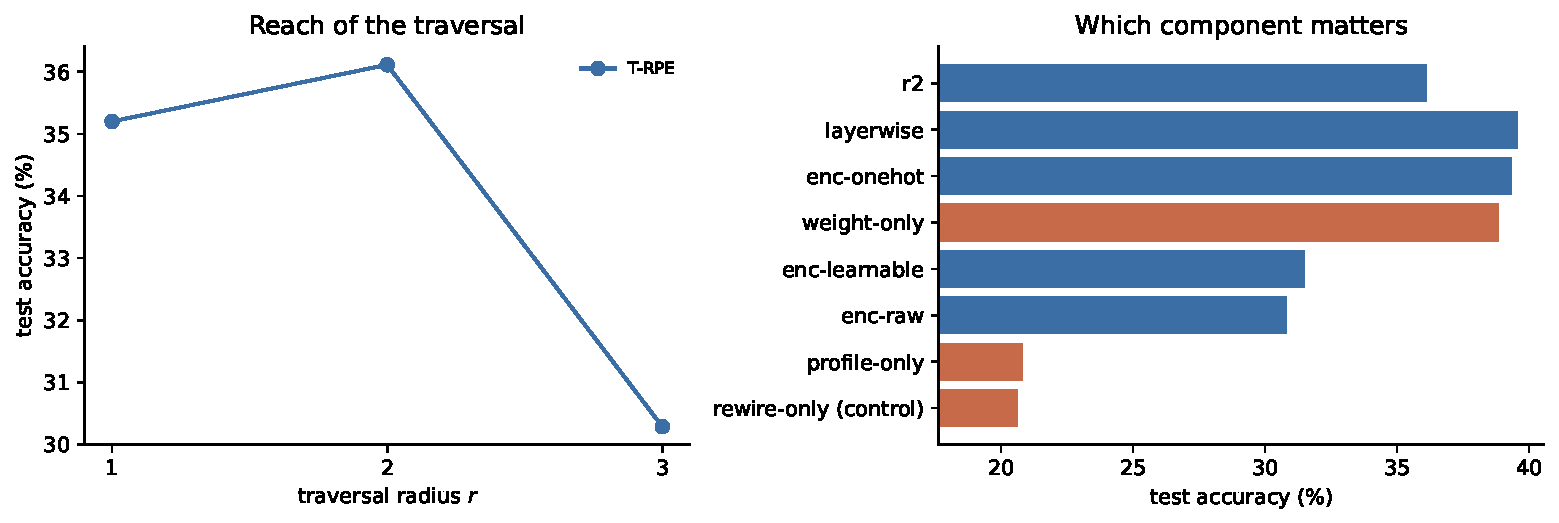
\includegraphics[width=\linewidth]{fig_ablations.pdf}
\caption{Ablations on GCN/CLUSTER, all variants at a matched budget. \textbf{rewire-only} and
the single-channel variants are highlighted. T-RPE at $r=2$ exceeds \textbf{rewire-only} by
$15.5$ points, so the gain is not attributable to the added connectivity alone.}
\label{fig:abl}
\end{figure}

\section{Limitations and Conclusion}

We studied traversal-based \emph{relative} positional encodings, which replace the anchor set
of absolute traversal encodings with a signal on node pairs, and require rewiring to reach a
sparse message-passing architecture.

Three limitations are structural. The method is bounded below 3-WL by
Proposition~\ref{prop:upper}, and strongly regular graphs are exactly what it cannot handle. It
has little to say on dense, short-diameter graphs, where nearly every pair sits at distance one
or two. And the radius $r$ is a cost knob rather than a free parameter, one we measure no
accuracy benefit from spending. Two further limitations are ours rather than the method's: our
M0 controls sit below published figures for these architectures on CLUSTER and CIFAR10-SP, so
comparisons here should be read between conditions and not against the literature, and
CIFAR10-SP ran at a single seed, too thin to support a claim about a two-point difference.

Our clearest results are negative, and we report them as findings. A relative encoding injected
as an edge weight or attention bias is provably inert under normalised aggregation
(Proposition~\ref{prop:cancel}) and empirically scores exactly chance where the theory says it
must. Our pre-registered prediction about where the encoding would help was wrong in the
opposite direction, because it assumed expressivity was the binding constraint on benchmarks
that turn out to have no 1-WL collisions at all. What survives both is one positive claim, and
it concerns injection rather than encoding: the same signal worth nothing under GCN is worth
$+21$ points under GAT. The channel a relative encoding is given matters more than the
information it carries, which suggests the useful question is not which structural signal to
compute, but which architectures can read one at all.

\bibliography{references}
\bibliographystyle{acl_natbib}

\appendix

\section{Distance diagnostics}
\label{app:diagnostic}
Figure~\ref{fig:dist} gives the per-dataset hop-distance histogram measured before any
training. Mean diameters are $6.0$ (CSL), $2.2$ (CLUSTER) and $8.5$ (CIFAR10-SP); CLUSTER
places $100\%$ of node pairs at distance $\le 2$, against $28.5\%$ for CSL and $22.8\%$ for
CIFAR10-SP. Edge blow-up $|E_r|/|E|$ is $2.9\times$ (CSL), $3.3\times$ (CLUSTER, already
saturated at $r=2$) and $2.8\times$ (CIFAR10-SP) at $r=2$, rising to $5.2\times$ and
$5.0\times$ at $r=3$ for CSL and CIFAR10-SP. This diagnostic is what the prediction in
\S\ref{sec:setup} was derived from, and it remains correct as a description of the graphs; what
it failed to predict is discussed in \S6.

\begin{figure}[h]
\centering
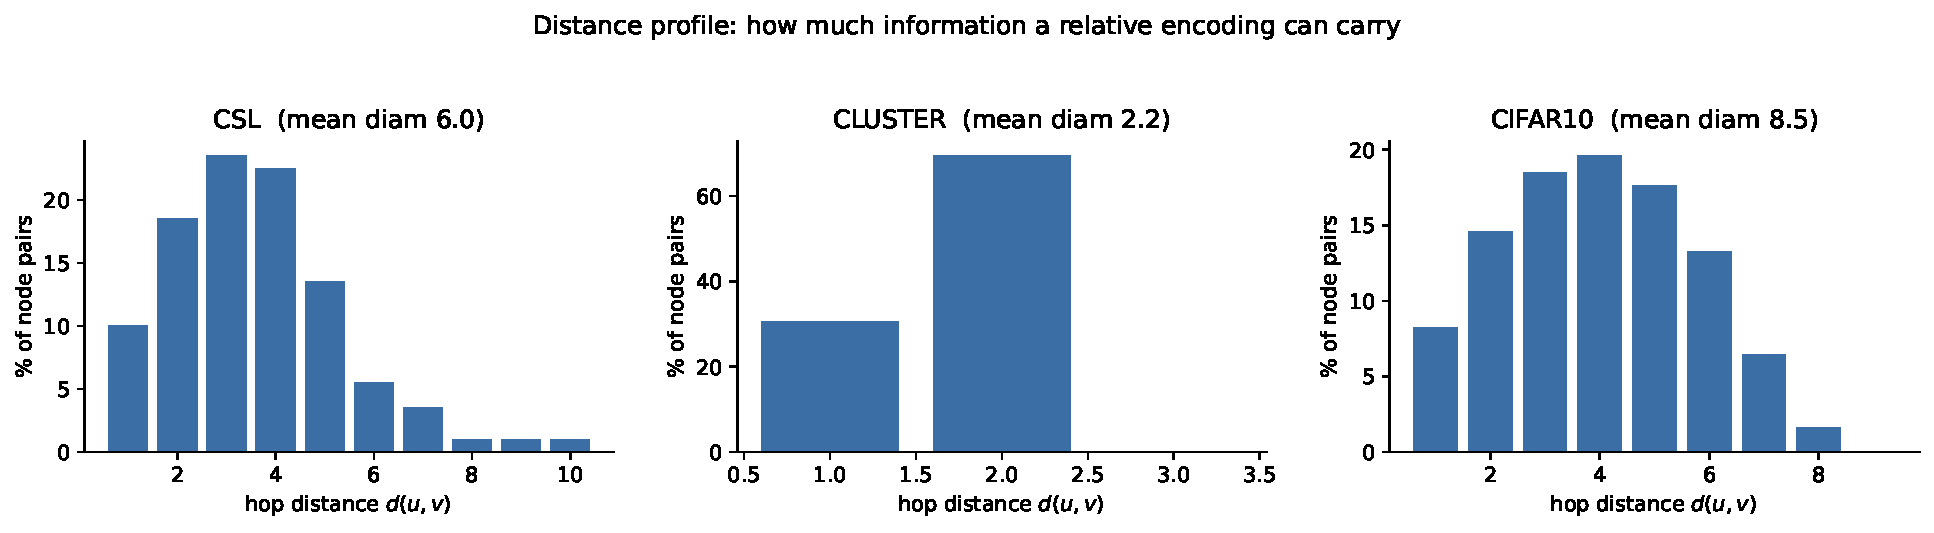
\includegraphics[width=\linewidth]{fig_distance_profile.pdf}
\caption{Hop-distance distribution per dataset, measured before training.}
\label{fig:dist}
\end{figure}

\section{Cost}
\label{app:cost}
Figure~\ref{fig:eff} gives preprocessing cost per graph against LapPE and RWPE, together with
the edge blow-up $|E_r|/|E|$. The blow-up, not the preprocessing, is the cost that recurs on
every epoch.

\begin{figure}[h]
\centering
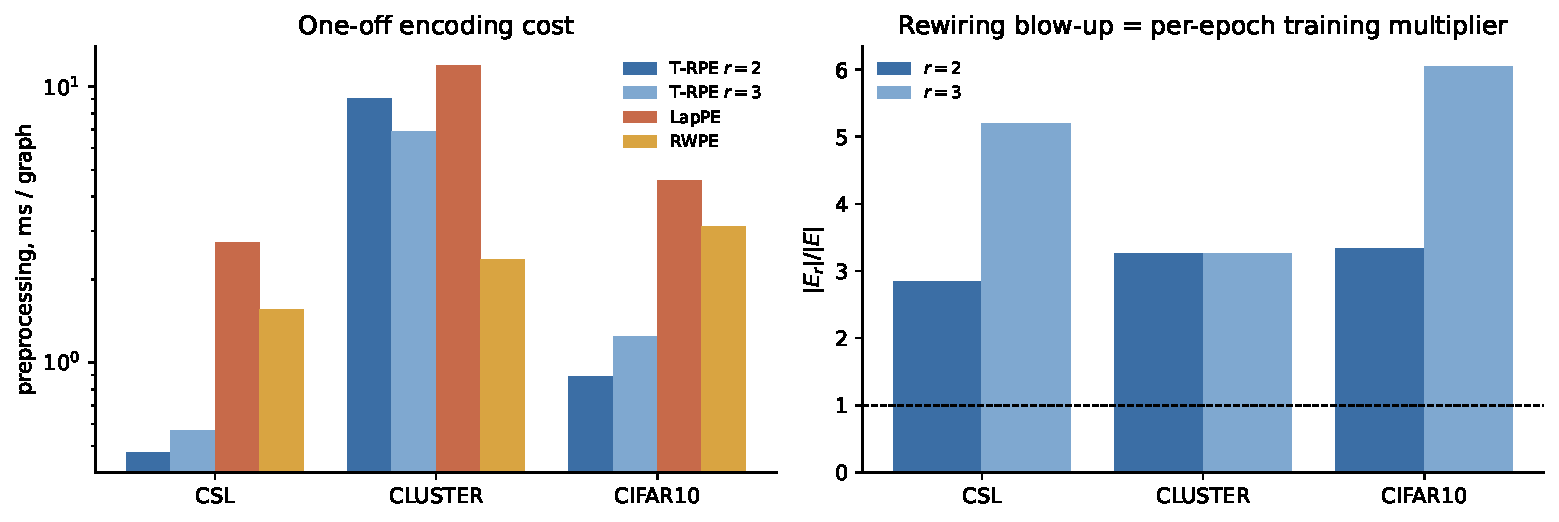
\includegraphics[width=\linewidth]{fig_efficiency.pdf}
\caption{Preprocessing cost per graph, and the edge blow-up $|E_r|/|E|$.}
\label{fig:eff}
\end{figure}

\section{Reproducibility}
Every experiment is a self-contained Colab notebook; each run writes one JSON file, and all
tables and figures in this paper are regenerated from those files by a single notebook. Code:
\textbf{[TODO: repository URL]}.

\end{document}
